\documentclass{jlreq}
\usepackage{graphicx}
\usepackage{amsmath,amssymb,mathtools,bm}
\usepackage{siunitx}
\sisetup{per-mode=symbol}
\usepackage{physics}
\usepackage{mhchem}
\usepackage{booktabs}
\usepackage{ascmac}
\usepackage{hyperref}
\hypersetup{colorlinks=true,linkcolor=black,urlcolor=blue,citecolor=black}
\usepackage{enumitem}
\usepackage{geometry}
\usepackage{caption}
\usepackage{makecell} % ← セル内改行・回転文字用


% ===== Title =====
\title{実体振り子の振動}
\author{学籍番号：2225091~~~~~~氏名 : 西亦 岳雄}

\begin{document}

\maketitle

% ===== 目的 =====

\begin{itembox}[l]{\large 実験の目的}

　実体振り子に関して, その重心と回転軸の線分距離を変化させ振動周期を計測し, 実体振り子における慣性モーメントと振動周期の関係性を調べる.

\end{itembox}


% ===== 原理 =====
\section*{1.原理}
　剛体とは, 外力がかかっても変形しない理想的な物体のことである. その剛体の運動を記述するため, 剛体の運動方程式を立てる. まず, ある剛体に軸を指し, その軸を指定するためにある2点を決める必要がある(この状態だと軸の周りに剛体が回転できてしまう). ここで, 剛体中のもう一点を指定し固定すれば剛体の刻々の動きを決めることができる. この一点は, $x,y,z$座標の三つのパラメータで決まるので, ここまでで9つのパラメータを指定する必要がある. さらに, 剛体を貫く2点と剛体の回転を止めるための残りの1点の互いの距離を一定とすれば, 自由度は6となり以下の6つの方程式を決めることができる.
\begin{align}
    M \ddot{\bm{r}}_G = \sum_{i=1}^{n} \bm{F}_i
\end{align}

\begin{align}
\bm{N} = \sum_{i=1}^{n} \bm{r}_i \times \bm{F}_i
\end{align}
ただし, $M$:剛体の質量, $\bm{r}_G$:剛体の重心の位置, $\bm{N}$:原点周りのトルク, $\bm{F}_i$:剛体中の$i$番目の質点が受ける外力である.
　剛体が固定された軸に貫かれている場合を考える. このときの剛体の自由度は1となるから, 必要な方程式は1つとなる. また, 剛体の運動は固定軸($z$軸)回りのトルクを用いて
\begin{align}
    N_z = \dot{L}_z
\end{align}
の式に従う. 剛体を微小な立方体に分割し$L_z$に関して足し上げると
\begin{align}
    L_z &= \sum_{i=1}^{n} (\bm{r}_i \times \bm{p}_i)\\
        &= \sum_{i=1}^{n} (\bm{r}_i \times m_i \dot{\bm{r}}_i)_z\\
        &\xrightarrow[\Delta V \to 0]{} \int_{}^{} dV[\bm{r} \times \rho(\bm{r})\dot{\bm{r}}]_z
\end{align}
ただし, $dV$:微小体積, $\rho(\bm{r})$:位置$\bm{r}$での密度である. ここからは, 円筒座標系を用いて(3)における角運動量を求める. 底面が$x,y$平面にあり, 中心軸を$z$軸とする円筒を考える. 底面の半径を$\xi$, $x$軸から$\xi$までの角度を$\theta$, $\xi, \theta, z$で指定される位置ベクトルを$\bm{r}$とする. すると,
\begin{align}
    \bm{r} \times \dot{\bm{r}} &= (\xi \bm{e}_{\xi} + z \bm{e}_z) \times \frac{d}{dt}(\xi \bm{e}_{\xi} + z \bm{e}_z)\\
                               &= (\xi \bm{e}_{\xi} + z \bm{e}_z) \times (\xi \dot{\bm{e}}_{\xi} + \xi \dot{\bm{e}}_{\xi} + \dot{z} \bm{e}_z)\\
                               &= (\xi \bm{e}_{\xi} + z \bm{e}_z) \times (\xi \dot{\bm{e}}_{\xi} + \xi \dot{\theta} \bm{e}_{} + \dot{z} \bm{e}_z)\\
                               &= (-z \xi \dot{\theta}) \bm{e}_{\xi} + (z \dot{\xi} - \xi \dot{z}) \bm{e}_{\theta} + ({\xi}^2 \dot{\theta}) \bm{e}_z
\end{align}
から, 角運動量の$z$成分は
\begin{align}
    L_z &= \int_{}^{} dV [\bm{r} \times \rho(\bm{r}) \dot{\bm{r}}]_z\\
        &= \int dV [\rho(\bm{r}) {\xi}^2 \dot{\theta}]\\
        &= \dot{\theta} \int_{}^{} dV [\rho(\bm{r}) {\xi}^2]
\end{align}
となり, $\int_{}^{} dV [\rho(\bm{r}) {\xi}^2]$の部分を$I_z$として慣性モーメントとする. (13)式について両辺を時間微分すると
\begin{align}
    \dot{L_z} = N_z = I_z \ddot{\theta}
\end{align}
が成り立つ.
　また, 運動エネルギー$K$に関して,
\begin{align}
    K &= \sum_{i=1}^{n} \frac{1}{2} m_i {\dot{\bm{r}}_i}^2\\
      &= \sum_{i=1}^{n} \frac{1}{2} m_i (\dot{\xi}_i \bm{e}_{\xi} + \xi_i \dot{\theta}_i \bm{e}_{\theta} + \dot{z_i} \bm{e}_z)^2\\
      &= \sum_{i=1}^{n} \frac{1}{2} m_i (\xi_i \dot{\theta}_i)^2\\
      & \xrightarrow[\Delta V \to 0]{} \int dV \frac{1}{2} \rho(\bm{r}) (\xi \dot{\theta})^2\\
      &= \frac{1}{2} I_z \dot{\theta}^2
\end{align}
が成り立つ.
　固定軸($z$軸)回りの慣性モーメントを$I_z$とすると
\begin{align}
    I_z &= \int dV \rho(\bm{r}) {\xi}^2\\
        &= \int \rho(\bm{r}) (x^2 + y^2)\\
        &= \int dV \rho(\bm{r}) ({x_G}^2 + {y_G}^2 + x'^2 + y'^2)\\
        &= Mh^2 + \int dV \rho(\bm{r}) (x'^2 + y'^2)
\end{align}
であり, $\int dV \rho(\bm{r}) (x'^2 + y'^2)$は$I_G$と表して, 重心回りの慣性モーメントとし, $h$は$z$軸から$z$軸に平行な軸までの距離である. これが, 重心$G$を通り$z$軸と平行な軸を通るときの慣性モーメントを表す平衡軸の定理である.




% ===== 図1 =====
\begin{figure}[hbtp]
  \centering
  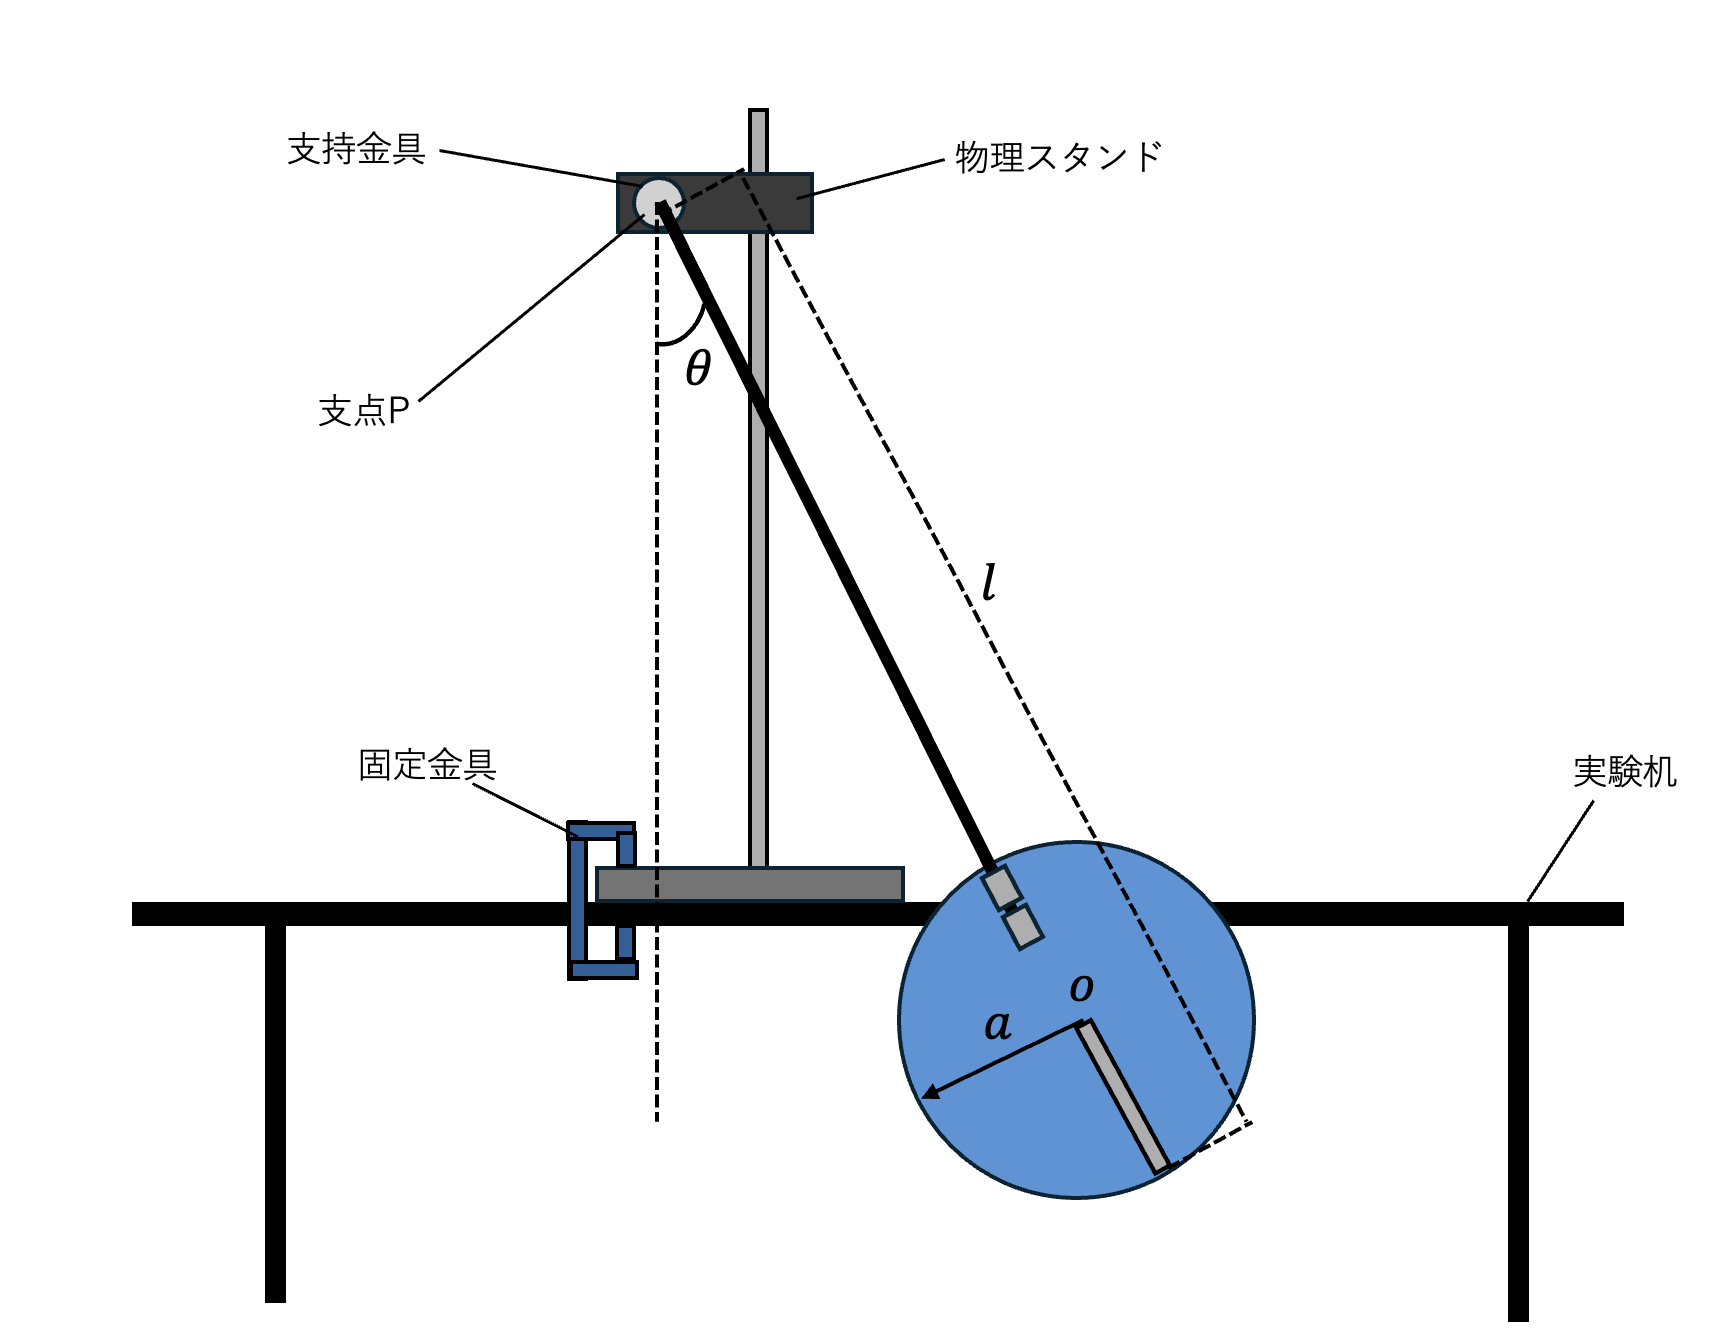
\includegraphics[width=1.0\linewidth]{image/setup1.png} % ← 拡張子・大文字小文字に注意！
  \caption{実験装置の概観}
\end{figure}








　図1にあるように, 半径$a$の円盤が支点Pから地面に垂直に下ろした軸の周りで振動する場合を考える. 円盤の重心Oと支点Pを貫く回転軸P(地面に平行)までの距離を$h$, O点で円盤に垂直な軸の周りの慣性モーメントを$I_z$, 円盤の質量を$M$, 支点Pから地面に垂直に下ろした垂線と円盤と支点Pを繋げた棒のなす角を$\theta$とする. 支点Pの周りでの円盤のトルクの方程式は
\begin{align}
    I \ddot{\theta} = N.
\end{align}
また, 重心にかかる重力のみがトルクに影響を与えるので
\begin{align}
    N &= \bm{r_G} \times m\bm{g}\\
      &= \xi \bm{e}_{\xi} \times mg(\cos \theta \bm{e}_{\xi} - \sin \theta \bm{e}_{\theta})\\
      &= -mg \xi \sin \theta.
\end{align}
(27)式がP点を通る軸の周りでの円盤の振動に関する方程式である. 振れ角が小さいとき($\theta \approx 0$)(27)式は
\begin{align}
    I \frac{d^2 \theta}{d t^2} = -Mgh\theta
\end{align}
と書ける. これより, 円盤の振動周期は
\begin{align}
    T = 2\pi \sqrt{\frac{I}{Mgh}}
\end{align}
となる. ここで平行軸の定理(23)を用いると
\begin{align}
    T = 2\pi \sqrt{\frac{1}{Mg}(\frac{I}{h} + Mh)}
\end{align}
を得る. 円盤に関するOの周りでの慣性モーメントは$I = \frac{M}{2}a^2$であるから, これを(30)に代入して
\begin{align}
    T = 2\pi \sqrt{\frac{1}{g} (\frac{a^2}{2h} + h)}.
\end{align}





% ===== 実験装置構成・方法 =====
\section*{2.実験装置構成・方法}
実験装置構成は図1にある通りで、実際の実験手順は以下である.

①円盤の質量を計測した.　→円盤の質量は500gであった.\par
②図1のように、実体振り子を組み立てた.\par
③回転軸Pを円盤の内側にするときは, 円盤の中心から回転軸までの距離$h$は円盤の直径から求めた半径$a$から, 回転軸までの距離を差し引いて求めた. \par
④円盤の中心Oから回転軸Pまでの距離を変えて, 振動周期を測定した. 円盤の振動の様子をスマートフォンで撮影し, その動画から5周期の経過時間を測定し, 平均周期を計算した. \par
⑤回転軸Pを円盤の外側に置くときは, まさに図1のように円盤の中心Oから回転軸までの距離$h$を円盤の数倍まで伸ばし, 振動周期$T$を測定した. 



% ===== 結果と解析 =====
\section*{3.結果と解析}
\subsection*{3.1円盤の内側}
まず, 円盤の内側に回転軸Pを置いたときをみる. 円盤の中心から回転軸までの距離$h$は表1にあるように$h\text{(m)} = 0.03, 0.06, 0.09, 0.12$の振動周期$T$を測定した. 表1が実際の実験値で, 円盤の中心から回転軸までの距離$h\text{(m)}$, 振動周期$T\text{(s)}$, $f_1 = \frac{a^2}{2h}$, $f_2 = h$, $f_1+f_2$をまとめたもの, また, 表2〜8が$h\text{(m)}$に対する振動周期$T\text{(s)}$, $f_1$, $f_2$, $f_1+f_2$をまとめたものである.


\begin{table}[htbp]
  \centering
  \caption{円盤内側の測定値}
  \renewcommand{\arraystretch}{1.2} % 行の高さ調整
  \setlength{\tabcolsep}{6pt}       % 列間隔調整
  \begin{tabular}{|c|c|c|c|c|c|}
    \hline
    $h\,(\mathrm{m})$ &
    $T\,(\mathrm{s})$ &
    $T^2\,(\mathrm{s}^2)$ &
    $f_1\,(\mathrm{m})$ &
    $f_2\,(\mathrm{m})$ &
    $f_1 + f_2\,(\mathrm{m})$ \\ \hline
    0.03 & 7.40 & 54.73 & 0.38 & 0.03 & 0.41 \\ \hline
    0.06 & 5.34 & 28.47 & 0.19 & 0.06 & 0.25 \\ \hline
    0.09 & 4.85 & 23.50 & 0.13 & 0.09 & 0.22 \\ \hline
    0.12 & 4.80 & 23.04 & 0.09 & 0.12 & 0.21 \\ \hline
  \end{tabular}
  \label{tab:disk_inner}
\end{table}




\begin{table}[htbp]
  \centering
  \caption{円盤内側の測定値（$h=0.03\,\mathrm{m}$ の場合）}
  \renewcommand{\arraystretch}{1.2} % 行の高さ調整
  \setlength{\tabcolsep}{6pt}       % 列間隔調整
  \begin{tabular}{|c|c|}
    \hline
    \textbf{$h\,(\mathrm{m})$} & \textbf{$T\,(\mathrm{s})$} \\ \hline
    0.03 & 7.40 \\ \hline
         & 7.37 \\ \hline
         & 7.28 \\ \hline
         & 7.41 \\ \hline
         & 7.53 \\ \hline
    平均 & 7.398 \\ \hline
  \end{tabular}
  \label{tab:disk_inner_0.03}
\end{table}




\begin{table}[htbp]
  \centering
  \caption{円盤内側の測定値（$h=0.06\,\mathrm{m}$ の場合）}
  \renewcommand{\arraystretch}{1.2} % 行の高さ調整
  \setlength{\tabcolsep}{6pt}       % 列間隔調整
  \begin{tabular}{|c|c|}
    \hline
    \textbf{$h\,(\mathrm{m})$} & \textbf{$T\,(\mathrm{s})$} \\ \hline
    0.06 & 5.25 \\ \hline
         & 5.32 \\ \hline
         & 5.30 \\ \hline
         & 5.43 \\ \hline
         & 5.38 \\ \hline
    平均 & 5.336 \\ \hline
  \end{tabular}
  \label{tab:disk_inner_0.06}
\end{table}



\begin{table}[htbp]
  \centering
  \caption{円盤内側の測定値（$h=0.09\,\mathrm{m}$ の場合）}
  \renewcommand{\arraystretch}{1.2} % 行の高さ調整
  \setlength{\tabcolsep}{6pt}       % 列間隔調整
  \begin{tabular}{|c|c|}
    \hline
    \textbf{$h\,(\mathrm{m})$} & \textbf{$T\,(\mathrm{s})$} \\ \hline
    0.09 & 4.82 \\ \hline
         & 4.85 \\ \hline
         & 4.80 \\ \hline
         & 4.87 \\ \hline
         & 4.90 \\ \hline
    平均 & 4.848 \\ \hline
  \end{tabular}
  \label{tab:disk_inner_0.09}
\end{table}


\begin{table}[htbp]
  \centering
  \caption{円盤内側の測定値（$h=0.12\,\mathrm{m}$ の場合）}
  \renewcommand{\arraystretch}{1.2} % 行の高さ調整
  \setlength{\tabcolsep}{6pt}       % 列間隔調整
  \begin{tabular}{|c|c|}
    \hline
    \textbf{$h\,(\mathrm{m})$} & \textbf{$T\,(\mathrm{s})$} \\ \hline
    0.12 & 4.77 \\ \hline
         & 4.80 \\ \hline
         & 4.78 \\ \hline
         & 4.82 \\ \hline
         & 4.83 \\ \hline
    平均 & 4.80 \\ \hline
  \end{tabular}
  \label{tab:disk_inner_0.12}
\end{table}




\begin{table}[htbp]
  \centering
  \caption{各 $h$ に対する $T^2$ の測定値}
  \renewcommand{\arraystretch}{1.2} % 行の高さ調整
  \setlength{\tabcolsep}{6pt}       % 列間隔調整
  \begin{tabular}{|c|c|}
    \hline
    \textbf{$h\,(\mathrm{m})$} & \textbf{$T^2\,(\mathrm{s^2})$} \\ \hline
    0.03 & 54.73 \\ \hline
    0.06 & 28.47 \\ \hline
    0.09 & 23.50 \\ \hline
    0.12 & 23.04 \\ \hline
  \end{tabular}
  \label{tab:T2_values}
\end{table}









\begin{table}[htbp]
  \centering
  \caption{各 $h$ に対する $f_1$ の測定値}
  \renewcommand{\arraystretch}{1.2} % 行の高さ調整
  \setlength{\tabcolsep}{6pt}       % 列間隔調整
  \begin{tabular}{|c|c|}
    \hline
    \textbf{$h\,(\mathrm{m})$} & \textbf{$f_1\,(\mathrm{m})$} \\ \hline
    0.03 & 0.375 \\ \hline
    0.06 & 0.188 \\ \hline
    0.09 & 0.125 \\ \hline
    0.12 & 0.094 \\ \hline
  \end{tabular}
  \label{tab:f1_values}
\end{table}







\begin{table}[htbp]
  \centering
  \caption{各 $h$ に対する $f_2$ の測定値}
  \renewcommand{\arraystretch}{1.2} % 行の高さ調整
  \setlength{\tabcolsep}{6pt}       % 列間隔調整
  \begin{tabular}{|c|c|}
    \hline
    \textbf{$h\,(\mathrm{m})$} & \textbf{$f_2\,(\mathrm{m})$} \\ \hline
    0.03 & 0.03 \\ \hline
    0.06 & 0.06 \\ \hline
    0.09 & 0.09 \\ \hline
    0.12 & 0.12 \\ \hline
  \end{tabular}
  \label{tab:f2_values}
\end{table}



\begin{table}[htbp]
  \centering
  \caption{各 $h$ に対する $f_1 + f_2$ の測定値}
  \renewcommand{\arraystretch}{1.2} % 行の高さ調整
  \setlength{\tabcolsep}{6pt}       % 列間隔調整
  \begin{tabular}{|c|c|}
    \hline
    \textbf{$h\,(\mathrm{m})$} & \textbf{$f_1 + f_2\,(\mathrm{m})$} \\ \hline
    0.03 & 0.780 \\ \hline
    0.06 & 0.435 \\ \hline
    0.09 & 0.340 \\ \hline
    0.12 & 0.308 \\ \hline
  \end{tabular}
  \label{tab:f1f2_values}
\end{table}



\subsubsection*{3.1.1　$h$ー$T^2$に関して}
表6をグラフにまとめたものが次の図2である. 



\begin{figure}[hbtp]
  \centering
  
\includegraphics[width=0.8\linewidth]{image/number1.png} % ← 拡張子・大文字小文字に注意！
  \caption{$h$(m)ー$T^2$(s$^2$)グラフ}
\end{figure}

実体振り子の振動周期は(30), (31)で表され, この両辺を2乗すると
\begin{align}
    T^2 = 4\pi^2 \frac{I + Mh^2}{Mgh} = \frac{4\pi^2 I}{Mgh} + \frac{4\pi^2 h}{g}
\end{align}

\begin{align}
    T^2 = \frac{4\pi^2}{g} (\frac{a^2}{2h} + h)
\end{align}
を得る. また, 図2と(32)から
\begin{align}
    T^2 = -333.47h + 57.447
\end{align}
の関係式を得る. 

\subsubsection*{3.1.2$h$ー$f_1, f_2, f_1+f_2$に関して}
表7〜9までをグラフにまとめたものが次の図3〜5である. 


\begin{figure}[hbtp]
  \centering
  
\includegraphics[width=0.8\linewidth]{image/number2.png} % ← 拡張子・大文字小文字に注意！
  \caption{$h$(m)ー$f_1$(m)グラフ}
\end{figure}

図3から得られる関係式は
\begin{align}
    f_1 = -3.02h + 0.42
\end{align}
である. 



\begin{figure}[hbtp]
  \centering
  
\includegraphics[width=0.8\linewidth]{image/number3.png} % ← 拡張子・大文字小文字に注意！
  \caption{$h$(m)ー$f_2$(m)グラフ}
\end{figure}




図4から得られる関係式は
\begin{align}
    f_2 = h
\end{align}
である. 



\begin{figure}[hbtp]
  \centering
  
\includegraphics[width=0.8\linewidth]{image/number4.png} % ← 拡張子・大文字小文字に注意！
  \caption{$h$(m)ー$f_1+f_2$(m)グラフ}
\end{figure}





図5から得られる関係式は
\begin{align}
    f_2 + f_1 = -5.04h + 0.84
\end{align}
である.

(33)を微分すると
\begin{align}
    \frac{dT^2}{dh} = 2T \frac{dT}{dh} = \frac{4\pi^2}{g}(-\frac{a^2}{2h^2} + 1)
\end{align}
となり, $\frac{dT}{dh} = 0$のとき, 周期$T^2$が極値$h = \frac{a}{\sqrt{2}}$をとることがわかる.



% ===== 3.2 =====
\subsection*{3.2　円盤の外側}
次に, 円盤の外側に回転軸Pを置いたときをみる. 円盤の中心から回転軸までの距離$h$は表10にあるように$h\text{(m)} = 0.55, 0.45, 0.35, 0.25$の振動周期$T$を測定した. 表10が表1同様に実際の実験値である. また, 表11〜18が$h$(m)に対する振動周期$T$(s), $f_1, f_2, f_1+f_2$をまとめたものである.


\begin{table}[htbp]
  \centering
  \caption{円盤外側の測定値}
  \renewcommand{\arraystretch}{1.2} % 行間を広げる
  \setlength{\tabcolsep}{6pt}       % 列間隔を調整
  \begin{tabular}{|c|c|c|c|c|c|}
    \hline
    \textbf{$h\,(\mathrm{m})$} & 
    \textbf{$T\,(\mathrm{s})$} & 
    \textbf{$T^2\,(\mathrm{s^2})$} & 
    \textbf{$f_1\,(\mathrm{m})$} & 
    \textbf{$f_2\,(\mathrm{m})$} & 
    \textbf{$f_1+f_2\,(\mathrm{m})$} \\ \hline
    0.55 & 7.69 & 59.17 & 0.02 & 0.55 & 0.57 \\ \hline
    0.45 & 6.93 & 48.08 & 0.03 & 0.45 & 0.48 \\ \hline
    0.35 & 6.29 & 39.61 & 0.03 & 0.35 & 0.38 \\ \hline
    0.25 & 5.54 & 30.71 & 0.05 & 0.25 & 0.30 \\ \hline
  \end{tabular}
  \label{tab:disk_outer}
\end{table}



\begin{table}[htbp]
  \centering
  \caption{円盤外側の測定値（$h=0.55\,\mathrm{m}$ の場合）}
  \renewcommand{\arraystretch}{1.2} % 行間調整
  \setlength{\tabcolsep}{6pt}       % 列間隔調整
  \begin{tabular}{|c|c|}
    \hline
    \textbf{$h\,(\mathrm{m})$} & \textbf{$T\,(\mathrm{s})$} \\ \hline
    0.55 & 7.66 \\ \hline
         & 7.65 \\ \hline
         & 7.72 \\ \hline
         & 7.75 \\ \hline
         & 7.68 \\ \hline
    平均 & 7.692 \\ \hline
  \end{tabular}
  \label{tab:disk_outer_0.55}
\end{table}




\begin{table}[htbp]
  \centering
  \caption{円盤外側の測定値（$h=0.45\,\mathrm{m}$ の場合）}
  \renewcommand{\arraystretch}{1.2} % 行間調整
  \setlength{\tabcolsep}{6pt}       % 列間隔調整
  \begin{tabular}{|c|c|}
    \hline
    \textbf{$h\,(\mathrm{m})$} & \textbf{$T\,(\mathrm{s})$} \\ \hline
    0.45 & 6.91 \\ \hline
         & 6.92 \\ \hline
         & 6.93 \\ \hline
         & 6.93 \\ \hline
         & 6.98 \\ \hline
    平均 & 6.934 \\ \hline
  \end{tabular}
  \label{tab:disk_outer_0.45}
\end{table}



\begin{table}[htbp]
  \centering
  \caption{円盤外側の測定値（$h=0.35\,\mathrm{m}$ の場合）}
  \renewcommand{\arraystretch}{1.2} % 行間調整
  \setlength{\tabcolsep}{6pt}       % 列間隔調整
  \begin{tabular}{|c|c|}
    \hline
    \textbf{$h\,(\mathrm{m})$} & \textbf{$T\,(\mathrm{s})$} \\ \hline
    0.35 & 6.23 \\ \hline
         & 6.24 \\ \hline
         & 6.35 \\ \hline
         & 6.34 \\ \hline
         & 6.31 \\ \hline
    平均 & 6.294 \\ \hline
  \end{tabular}
  \label{tab:disk_outer_0.35}
\end{table}





\begin{table}[htbp]
  \centering
  \caption{円盤外側の測定値（$h=0.25\,\mathrm{m}$ の場合）}
  \renewcommand{\arraystretch}{1.2} % 行間調整
  \setlength{\tabcolsep}{6pt}       % 列間隔調整
  \begin{tabular}{|c|c|}
    \hline
    \textbf{$h\,(\mathrm{m})$} & \textbf{$T\,(\mathrm{s})$} \\ \hline
    0.25 & 5.54 \\ \hline
         & 5.57 \\ \hline
         & 5.51 \\ \hline
         & 5.52 \\ \hline
         & 5.57 \\ \hline
    平均 & 5.542 \\ \hline
  \end{tabular}
  \label{tab:disk_outer_0.25}
\end{table}




\begin{table}[htbp]
  \centering
  \caption{各 $h$ に対する $T^2$ の測定値（円盤外側）}
  \renewcommand{\arraystretch}{1.2} % 行間調整
  \setlength{\tabcolsep}{6pt}       % 列間隔調整
  \begin{tabular}{|c|c|}
    \hline
    \textbf{$h\,(\mathrm{m})$} & \textbf{$T^2\,(\mathrm{s^2})$} \\ \hline
    0.55 & 59.17 \\ \hline
    0.45 & 48.08 \\ \hline
    0.35 & 39.61 \\ \hline
    0.25 & 30.71 \\ \hline
  \end{tabular}
  \label{tab:disk_outer_T2}
\end{table}




\begin{table}[htbp]
  \centering
  \caption{各 $h$ に対する $f_1$ の測定値（円盤外側）}
  \renewcommand{\arraystretch}{1.2} % 行間調整
  \setlength{\tabcolsep}{6pt}       % 列間隔調整
  \begin{tabular}{|c|c|}
    \hline
    \textbf{$h\,(\mathrm{m})$} & \textbf{$f_1\,(\mathrm{m})$} \\ \hline
    0.55 & 0.02 \\ \hline
    0.45 & 0.03 \\ \hline
    0.35 & 0.03 \\ \hline
    0.25 & 0.05 \\ \hline
  \end{tabular}
  \label{tab:disk_outer_f1}
\end{table}





\begin{table}[htbp]
  \centering
  \caption{各 $h$ に対する $f_2$ の測定値（円盤外側）}
  \renewcommand{\arraystretch}{1.2} % 行間調整
  \setlength{\tabcolsep}{6pt}       % 列間隔調整
  \begin{tabular}{|c|c|}
    \hline
    \textbf{$h\,(\mathrm{m})$} & \textbf{$f_2\,(\mathrm{m})$} \\ \hline
    0.55 & 0.55 \\ \hline
    0.45 & 0.45 \\ \hline
    0.35 & 0.35 \\ \hline
    0.25 & 0.25 \\ \hline
  \end{tabular}
  \label{tab:disk_outer_f2}
\end{table}




\begin{table}[htbp]
  \centering
  \caption{各 $h$ に対する $f_1 + f_2$ の測定値（円盤外側）}
  \renewcommand{\arraystretch}{1.2} % 行間調整
  \setlength{\tabcolsep}{6pt}       % 列間隔調整
  \begin{tabular}{|c|c|}
    \hline
    \textbf{$h\,(\mathrm{m})$} & \textbf{$f_1 + f_2\,(\mathrm{m})$} \\ \hline
    0.55 & 0.57 \\ \hline
    0.45 & 0.48 \\ \hline
    0.35 & 0.38 \\ \hline
    0.25 & 0.30 \\ \hline
  \end{tabular}
  \label{tab:disk_outer_f1f2}
\end{table}


\subsection*{3.2.1　$h$ー$T^2$に関して}
表15をグラフにまとめたものが図6である. 振動周期は円盤の内側に回転軸を置いたときと同様に(33)で書ける.

\begin{figure}[hbtp]
  \centering
  
\includegraphics[width=0.8\linewidth]{image/number5.png} % ← 拡張子・大文字小文字に注意！
  \caption{$h$(m)ー$T^2$(s$^2$)グラフ}
\end{figure}

図6の関係式は

\begin{align}
    T^2 = 93.83h + 6.86
\end{align}
である.


\subsubsection*{3.2.2　$h$ー$f_1, f_2, f_1+f_2$に関して}
表16〜18をグラフにまとめたものが次の図7〜9である.

\begin{figure}[hbtp]
  \centering
  
\includegraphics[width=0.8\linewidth]{image/number6.png} % ← 拡張子・大文字小文字に注意！
  \caption{$h$(m)ー$f_1$(m)グラフ}
\end{figure}



図7の関係式は
\begin{align}
    f_1 = -0.08h + 0.063
\end{align}
である.



\begin{figure}[hbtp]
  \centering
  
\includegraphics[width=0.8\linewidth]{image/number7.png} % ← 拡張子・大文字小文字に注意！
  \caption{$h$(m)ー$f_2$(m)グラフ}
\end{figure}



図8の関係式は
\begin{align}
    f_2 = h
\end{align}
である.

\begin{figure}[hbtp]
  \centering
  
\includegraphics[width=0.8\linewidth]{image/number8.png} % ← 拡張子・大文字小文字に注意！
  \caption{$h$(m)ー$f_1+f_2$(m)グラフ}
\end{figure}



図9の関係式は
\begin{align}
    f_1+f_2 = 0.92h + 0.06
\end{align}



















% ===== 考察 =====
\section*{4.考察}
\subsection*{4.1回転軸を円盤内側に置いたとき}
図2から, $T^2$は$h$に対して, 負の傾きをもつことがわかる. また, (33)式より, $h$が増加すると$\frac{a^2}{2h}$が減少するので, (29)も合わせてみると慣性モーメント$I$は小さくなりかつ振動周期も短くなる. これより, 実験値より得られた関係式$T^2 = -333.47h + 57.447$は理論式に傾向として一致することがわかる.\par

実体振り子では, 振動周期が
\begin{align}
  T = 2\pi \sqrt{\frac{1}{g} (\frac{a^2}{2h} + h)}
\end{align}
と書けるが, 単振り子の場合は
\begin{align}
  T = 2\pi \sqrt{\frac{l}{g}}
\end{align}
と書ける. ここで$l$は支点から振り子球の重心までの距離で, $l$が大きいほど周期が長くなることがわかる. $h$が小さいとき, つまり, 支点Pが重心に限りなく近いときには$T$が増加し, 対して$h$が大きいとき$T \simeq 2\pi \sqrt{\frac{h}{g}}$となって単振り子と近い形での依存性が確認できる.\par

重力加速度$g$を実験値から求める. 理論式は
\begin{align}
  T^2 = A(f_1+f_2)
\end{align}
となり, この実験値表は


% Table generated by Excel2LaTeX from sheet '円盤内側'
\begin{table}[htbp]
  \centering
  \caption{円盤内側における $(f_1 + f_2)$ と $T^2$ の関係}
  \begin{tabular}{cc}
    \toprule
    \textbf{$f_1 + f_2$ (m)} & \textbf{$T^2$ (s$^2$)} \\
    \midrule
    0.41 & 54.73 \\
    0.25 & 28.47 \\
    0.22 & 23.50 \\
    0.21 & 23.04 \\
    \bottomrule
  \end{tabular}
  \label{tab:disk_inner}
\end{table}
となる. グラフは


\begin{figure}[hbtp]
  \centering
  
\includegraphics[width=0.8\linewidth]{image/number9.png} % ← 拡張子・大文字小文字に注意！
  \caption{$T^2$(s$^2$)ー$f_1+f_2$(m)グラフ}
\end{figure}


図10から得られる関係式は
\begin{align}
  T^2 = 165.28(f_1+f_2) - 12.24
\end{align}
である. これから重力加速度$g$を求めると
\begin{align}
  g = \frac{4\pi^2}{A}
\end{align}
より, $g = \frac{39.47}{165.28} \simeq 0.239$(m/s$^2$)と誤差の割合が97.6％にもなり理論値である9.8(m/s$^2$)と大きくずれた. これは, 円盤の内側に回転軸を置くと, 支点Pが重心に近くなり慣性モーメント$I$の影響が大きく出ることに起因すると考えられる.\par

次に, 重力加速度$g$を求める際, 精度を高める工夫について考える. 1つには, $\sin \theta \simeq \theta$で近似するわけであるが, 円盤を手から離すとき(初期の振れ角)をできる限り小さくすることで理論式との齟齬を少なくすること. 2つには, 測定回数を大幅に増やすことである. 図5をみると, どのプロットも近似直線から離れていて, 適した比例関係が得られているとは考えられない. プロット数を増やすことで, より近似直線に近い結果が得られると考えた.





% ===== 概括 =====
\section*{5.概括}
\section*{まとめ}
今回の実験では, 実体振り子の振動周期を測定し
\begin{align}
  T^2 = \frac{4\pi^2}{g}(\frac{a^2}{2h} + h)
\end{align}
から重力加速度$g$を求めた. また, 測定の結果から, $T^2$と$f_1 + f_2$に関して大まかな比例関係を確認することができ, 実体振り子の周期的運動が理論式にある程度従うことがわかった. 一方で, 求めた重力加速度$g$は大幅に小さい結果となった. この改善策として, 初期振れ角を小さくすること, また測定回数を増やしてより適した比例関係を得ることを提案した.


\end{document}





